\documentclass[12,fleqn]{article}
\hoffset=0.0cm \voffset= 0cm \textwidth=14.cm \textheight=20cm

\usepackage{a4wide,caption,epsfig,url}
\usepackage{fancyhdr}
\usepackage{todonotes}
\usepackage{fleqn}
\usepackage{graphicx}
\usepackage{subcaption}
\usepackage{hyperref}
\usepackage{todonotes}
\usepackage{amsthm}
\usepackage{amsfonts}
\usepackage{amsmath}
\usepackage{amssymb}
\usepackage{verbatim}
%\usepackage{makeidx}
\usepackage{latexsym}
\usepackage{fancyhdr}
\usepackage{tikz}
\usepackage{float}
\usepackage{cancel}
\usepackage{apacite}
\usepackage{algorithm}
\usepackage[noend]{algpseudocode}
\usepackage{multirow}
\graphicspath{ {images/} }
%\usepackage{natbib}


%\pagestyle{fancy}


\theoremstyle{definition}
\newtheorem{defi}{Definition}
\newtheorem{al}[defi]{Algorithm}
\newtheorem{id}[defi]{Idea}

\theoremstyle{plain}
\newtheorem{thm}[defi]{Theorem}
\newtheorem{lem}[defi]{Lemma}
\newtheorem{cor}[defi]{Corollary}
\newtheorem{prop}[defi]{Proposition}
\newtheorem{conj}[defi]{Conjecture}
\newtheorem{qn}[defi]{Question}

%pseudocode
%\makeatletter
%\def\BState{\State\hskip-\ALG@thistlm}
%\makeatother



\setlength{\headheight}{15pt}
\lhead{Summer VRES}
\rfoot{}
\rhead{Ryan Kelly}
\cfoot{\thepage}
\lfoot{}

%\title{SEF VRES \\
%Topics in Computational Bayesian Statistics}
%\author{Ryan Kelly}
\bibliographystyle{apacite}
\begin{document}
%\maketitle

\begin{titlepage}
\vspace*{5em}
\begin{center}
\Large{Queensland University of Technology}\\[0.5em]
%include qut image

\includegraphics[scale = 0.3]{qut.jpg}\\
\huge{Approximate Bayesian Computation with Independent Proposals for a g-and-k Model }\\[0.2em]
\large{VRES report}\\[2em]
\large{
Ryan Kelly 	n9751041 \\[0.1em]
Supervisor: Dr Christopher Drovandi \\
\vspace{5mm}
November 2017 - February 2018
}
\end{center}
\vspace*{\fill}
%\large{Abstract}
\paragraph{}
Approximate Bayesian Computation (ABC) methods are useful when the likelihood is unavailable but simulation from the model is straightforward. Approximate Bayesian Computation (ABC) has been shown to be effective in targeting the posterior of a g-and-k distribution. The g-and-k model is a quantile function that has an expensive likelihood function while model simulation is simple through the inversion method making it ideal for ABC. A key step in ABC is the proposal of a new parameter. An inefficient proposal method will suggest bad parameter values which increases the computation time.  The most common method to propose a new parameter given a current value is a normal random walk. However, an independent proposal method allows the possibility to recycle all proposed parameters which can be used to achieve a much higher effective sample size (ESS). The main aim of this report was to implement an independent proposal method for a g-and-k model and compare its approximate posterior to a standard random walk method. The ABC method used is the Sequential Monte Carlo (SMC) replenishment algorithm. The SMC with independent proposals was applied first to a trivial example of a binomial distribution and then to the more complex g-and-k model. In the two examples, multiple runs were made that gave the approximate posterior of the model. Both proposal methods gave approximately the same posteriors justifying the potential use of the independent proposal method. It was found that for (N = 800) particles that the independent proposal method took roughly ten times longer to compute compared to the random walk for a single dataset. However, further work that uses the saved independent proposals to improve the ESS could make the independent proposal approach more efficient compared to the standard random walk. Ultimately, this report makes the first step by implementing independent proposals for the g-and-k model.
\par
\end{titlepage}


\tableofcontents

\section{Introduction}
\paragraph{}
Bayesian statistics provides a framework for a statistical inference for quantifying the uncertainty of unknowns based on information pre and post data collection. This information is captured in the posterior distribution, which is a probability distribution over the space of unknowns given the observed data. The posterior distribution has the form:
\par
\begin{equation*}
\pi(\theta|y) \propto f(y|\theta)\pi(\theta)
\end{equation*}

\paragraph{}
 The ability to make inferences based on the posterior essentially amounts to the ability to efficiently simulate from the posterior distribution, which can generally not be done perfectly in practice. Approximate Bayesian computation (ABC) can be used when the likelihood is unavailable analytically or computationally but simulation from the model is straightforward. This is done through instead targeting the approximate posterior which has the form:
\par

\begin{equation*}
\pi_\epsilon(\theta, x|y) \propto K_\epsilon (\rho(y,x))f(x|\theta)\pi(\theta)
\end{equation*}

\paragraph{}
A more comprehensive outline of ABC algorithms is covered in Section 3, to quickly summarise, initially some summary statistic is generated from the observed dataset. For ever proposed $\theta$ a new dataset is simulated with an associated summary statistic. The observed and simulated datasets are then compared through a discrepancy function using the summary statistics. Finally, the proposed parameter is accepted if the discrepancy function gives a result smaller than some $\epsilon$.
\par
\paragraph{}
There are effectively two sources of error in ABC approximation. The first is from the summary statistic not being sufficient. The second source of error is the necessary introduction of a tolerance $\epsilon$. For ABC to be successull, we require $\epsilon$ to be small, but this requires increased computation. It is therefore necessary to have an efficient ABC algorithm to sample for the ABC posterior when $\epsilon$ is small.
\par

\paragraph{}
While this report will briefly touch on both the ABC rejection and Markov Chain Monte Carlo (MCMC) ABC algorithms the focus will be on Sequential Monte Carlo (SMC) ABC,  in particular the replenishment SMC ABC algorithm of \citeA{macroparasitesmc}. SMC is an extension of importance sampling where a sequence of target distributions construct a path between the initial distribution and the final distribution.
\par

\paragraph{}
While this approach tends to be more efficient than ABC rejection, it has the drawback that the method must be re-run and tuned for each new dataset or summary statistic selection. Additionally, only the final accepted samples from the last target distribution is typically kept from SMC ABC with no use for proposals from previous iterations.  It has been theorised by \citeA{quteprints101729} that making use of all proposals would substantially increase the ESS. To be able to use all of these proposals an approach that uses independent proposals is required instead of the standard normal walk proposals. 
\par

\paragraph{}
The aim of this report is to implement SMC ABC using independent proposals on a g-and-k model. The approximate posterior will then be compared against an SMC ABC with random walk proposals method. This is the first step towards the ultimate goal of using the independent proposals saved to increase the ESS. 
\par

\paragraph{}
Independent proposals have the advantage that they can result in uniformly ergodic Markov chains, as opposed to typical geometric ergodicity achieved by random walk proposals \cite{tierney}. A by-product of using an independent proposal method was investigated by \citeA{quteprints101729}  concerning the possibility of considering various importance sampling (IS) estimators of the marginal likelihood using all proposals in the SMC process.
\par



\section{Bayesian Statistics Background}
\subsection{Posterior} 
\paragraph{}
Bayesian statistics is based on Bayes' Theorem:
\begin{equation*}
Pr(B|A) = \frac{Pr(A|B) Pr(B)}{Pr(A)}
\end{equation*}
Here Pr(B) is the prior, which is the probability density that expresses one's beliefs before accounting for evidence. Pr(A$|$B) gives the likelihood of getting values A given the parameters B. Of key interest in regards to ABC is Pr(B$|$A) which is the posterior which is the probability of the parameter B given the evidence A. The difficulties in computing the posterior becomes clearer when considering a general form of Bayes theorem:
\begin{equation*}
\pi(\theta|\boldsymbol{y}) = \frac{f(\boldsymbol{y}|\theta) \pi(\theta)}{\int_\Theta f(\boldsymbol{y} | \theta) \pi(\theta) d\theta}
\end{equation*}
where $\pi$ is the prior/posterior distributions and $f$ is the likelihood function. Clearly the integral on the denominator can become very difficult to compute. It follows that several innovations have been made to not sample directly from the posterior, $\pi(\theta|\boldsymbol{y})$. A key initial innovation was the Monte Carlo method with the focus in this report being on the Metropolis-Hastings Algorithm. This is a method of Markov Chain Monte Carlo (MCMC) which can be applied in ABC. 
\par


\subsection{Metropolis-Hastings}
\paragraph{}
MCMC was first introduced by \citeA{metropolis}. This class of algorithms allows sampling from a probability distribution through constructing a Markov Chain that has the desired distribution as its equilibrium distribution. It follows that the target can be set to the posterior distribution $\pi(\boldsymbol{\theta} | \boldsymbol{Y})$. Hastings expanded on Metropolis's original paper to include non-symmetrical proposal distributions which led to the Metropolis-Hastings algorithm \cite{hastings}. The algorithm as outlined in \citeA{drovandilecturenotes} is as follows:
\begin{algorithm}
\caption{The Metropolis-Hastings Sampler}
\begin{algorithmic}[1]
\State Initialise $\theta^0$
\State { \textbf{for} t = 1 \textbf{to} \textit{T} \textbf{do} }
\State     Given the current parameter value $\theta = \theta^t$, propose $\theta$' 	from some proposal distribution $q(\theta'|\theta)$
\State Calculate acceptance probability $\alpha(\theta \rightarrow \theta') = min\left( 1, \frac{\pi(\theta')q(\theta|\theta')}{\pi(\theta)q(\theta'|\theta)} \right) $
\State Set $\theta^{t+1} = \theta'$  with probability  $\alpha(\theta' \rightarrow \theta)$, otherwise set $\theta^{t+1} = \theta^t$
\State \textbf{end for}
\end{algorithmic}
\end{algorithm}
\par



\paragraph{}
Two different approaches to the proposal distribution were considered in this report. The first was a normal random walk which is popular for a continuous parameter space. A random walk is a sequence of random values which satisfy:
\begin{equation*}
\theta^{t+1} = \theta^t + \epsilon_t
\end{equation*}
Where $\epsilon$ is distributed by a normal distribution. Clearly this is distributed symmetrically which means it is not needed to be computed in the Metropolis-Hastings ratio.
\par

\paragraph{}
A second approach is an independent proposal, where $q(\theta'|\theta) = g(\theta').$ Unlike the random walk approach, the proposed parameter value is independent of the current state of the chain, and the Markov chain explores the neighbourhood of a sensible proposal already computed. This approach is useful if there is both a low number of dimensions (such as both examples considered in this report) and sensible proposals.
\par


\subsection{Sequential Monte Carlo}
\paragraph{}
The focus in this report will be the SMC algorithm of \citeA{chopin} which was one of the first SMC algorithms for static models.
Sequential Monte Carlo (SMC) can be seen as an extension of importance sampling.  Here we require a sequence of slowly evolving distributions, $p_0(x), p_1(x), \ldots, p_T(x)$, where $p_0$ is easy to sample from directly and $p_T$ is the ultimate target distribution, which is hard to sample from directly. The method involves traversing a set of $N$ weighted samples through the sequence of iteratively applying the following steps: re-weighting (importance sampling), re-sampling, move.
\par

\section{ABC Algorithms}
\subsection{ABC posterior}
\paragraph{}
Approximate Bayesian Computation offers a way to approximately compute the posterior when the likelihood is intractable through instead targeting the approximate posterior. The approximate posterior has the form:
\begin{equation*}
\pi_\epsilon(\theta, x|y) \propto K_\epsilon (\rho(y,x))f(x|\theta)\pi(\theta)
\end{equation*}
 
\paragraph{}
Where the discrepancy function, $\rho(y,x)$ compares the observed data, y, with the simulated data, x. Essentially this measures how similar the two datasets are. This comparison is usually done on the basis of a summary statistic, $S(y)$. The choice of summary statistic is a compromise between dimensionality and information loss. $K_\epsilon (\rho(y,x))$ is a weighting function that gives higher weight the closer the simulated summary statistic is the observed summary statistic. One common choice is to set $K_\epsilon (\rho(y,x)) = 1(\rho(y,x) \leq \epsilon)$ where $1(\cdot)$ is the indicator function. Finally, $ f(x|\theta)$ is the likelihood but now evaluated on the simulated data. In practice this computation does not need to be performed. This gives a joint distribution over $\theta$ and the simulated data $x$. ABC algorithms sample over this joint density, so it possible to sample from the marginal $\theta$ by simply ignoring the $x$ samples.
\par

%Considered in this report is generating summary statistics from an auxiliary model. 

\paragraph{}
The choice of $\epsilon$ in ABC rejection represents a trade-off between accuracy and computational effort. A smaller value of $\epsilon$ forces a closer match between observed and simulated data (and leads to higher accuracy) but will decrease the acceptance rate meaning that more computation is required to obtain the desired number of samples. There are effectively two sources of error in the ABC approximation. The first is from the summary statistic not being sufficient. The second is the necessary introduction of the tolerance $\epsilon$.
\par

\paragraph{}
There is no universally best accepted approach to select a summary statistic. In this report we will mainly consider summary statistics from auxiliary models.  
 In indirect inference, estimation of $\theta$ is facilitated by specifying an alternative (auxiliary) parametric model with parameter $\phi$. It is important that such a model has a tractable likelihood function. One could use the parameter estimates (e.g. MLE) of this auxiliary model fitted to the observed data, $\phi(y)$, as a summary statistic for ABC. The simulated summary statistic comes from fitting the auxiliary model to data simulated from the 'true' model, $\phi(x).$ If there is no analytic expression for the auxiliary MLE, this approach can be expensive as it requires fitting the auxiliary model to each dataset simulated from the 'true' model.
\par

\paragraph{}
As an alternative we can use the score of the auxiliary model as the summary statistic:
\begin{equation}
S_A(y, \phi) =\left( \frac{\partial \log \ p_A(y|\phi)}{\partial \phi_1}, \cdots, \frac{ \partial \log \ p_A(y|\phi)}{\partial \phi_{dim(\phi)} } \right)^T ,
\end{equation}
In order to use this, we need a parameter value for $\phi$. We can choose $\phi(y)$ for example. With this approach, there is a massive improvement in computation time if there is analytic expression for the score as we only need to fit the auxiliary model to observed data once before the ABC analysis. 
\par


\subsection{ABC Rejection}
\paragraph{}
The first ABC algorithm developed was ABC rejection \cite{Beaumont}. In this approach parameter values are proposed from the prior distribution, $\theta \sim \pi(\cdot)$. Because the ABC target is defined over the joint space of the parameter $\theta$ and the simulated data $x$, it is necessary to devise an importance distribution that exists over the same space.
$ g(\theta, x) = g(\theta)f(x|\theta)$
where g($\cdot$) is some general proposal over the $\theta$ space. The simulated data x gets drawn from the likelihood conditional on the proposed $\theta$. To implement importance sampling, a large sample of size $M$ is generated from the importance distribution, $ \{\theta_i, x_i\}^M_{i=1} \overset{iid}{\sim} g(\theta, x)$. This size $M$ is determined by computational constraints. Then in order to ensure that the samples are from $\pi_\epsilon$ the following weighting must be performed:
\begin{equation*}
w_i = \frac{K_\epsilon(\rho(y,x)) \cancel{f(x_i | \theta_i)} \pi(\theta_i)}{g(\theta_i)\cancel{f(x_i | \theta_i)}}
\end{equation*}
where the target density is taken and divided by the importance distribution. Note that the likelihood terms cancel and no intractable terms are left.
If the proposal distribution is set to be equal to the prior $g(\theta) = \pi(\theta)$ then the terms cancel and we are just left with the weight function is $K_\epsilon(\rho(y,x)) = 1(\rho(y,x) \leq \epsilon)$ which means $w_i$ is either 0 or 1.

\hfill\break
ABC rejection has the strength over other ABC algorithms that it is useful for testing different sets of summary statistics \cite{nunes} or analysing multiple datasets from same model since the $M$ prior predictive simulations can be re-used (i.e. they are independent of the actual observed data). However, ABC rejection has the drawback of being inefficient if the posterior is different to the prior leaving it not effective for most applications. To achieve a reasonable computation time in this case would lead to a too high $\epsilon$ which would mean the ESS would be too low. 
\par

\subsection{MCMC ABC}
\paragraph{}
To overcome the problem outlined for ABC rejection \cite{marjoram} developed an MCMC algorithm without likelihoods. This approach builds on the Metropolis-Hastings ratio outlined in Section 2.2. MCMC is based on the idea of constructing a Markov chain whose limiting distribution is given by the target distribution of interest, here the ABC posterior, $\pi_\epsilon$. As in importance sampling, we require a proposal distribution on the joint space $\theta$ and $x$. However, our proposed value is allowed to depend on the state of the Markov chain, $q(\theta^*, x^* | \theta, x)$. Here we select $q(\theta^*, x^* | \theta, x)$ = $f(x^* | \theta^*)q(\theta^* | \theta)$ where $q(\theta^* | \theta)$ is an arbitrary proposal over the $\theta$ space and the term $f(x^* | \theta^*)$ tells us we must draw simulated data from the likelihood conditional on the proposed $\theta^*$. This choice leads to the following Metropolis-Hastings ratio:
\par
\begin{equation*}
r= \frac{K_\epsilon(\rho(y,x^*))\cancel{f(x^* | \theta^*)}\pi(\theta^*)q(\theta|\theta^*)\cancel{f(x|\theta)}}{K_\epsilon(\rho(y,x))\cancel{f(x| \theta)}\pi(\theta^*)q(\theta^*|\theta)\cancel{f(x^*|\theta^*)}}
\end{equation*}
\paragraph{}
Where all the intractable likelihood terms have cancelled out. Additionally, if the proposal distribution is symmetric this also does not need to be computed. 
\par
\paragraph{}
Many variants of MCMC have been developed to increase efficiency. Considered here will be the use of 'early rejection' within MCMC ABC developed by \citeA{picchini} which can be applied when using the uniform kernel weighting function. The advantage of this method is that proposed parameters can be rejected without having to simulate any data. The idea behind the early rejection is computing the Metropolis-Hastings ratio without the indicator function (which requires simulation) first. The indicator is only need on the denominator for the proposed parameter as the value for the current value in the chain is guaranteed to be 1 as it was accepted.
\begin{equation*}
s = \frac{\pi(\theta^*) q(\theta^{i - 1} | \theta^*)}{\pi(\theta^{i - 1}) q(\theta^* | \theta^{i - 1})}
\end{equation*}
Then draw $u \sim U(0,1)$ and if $u > s$ then the parameter $\theta*$ can be rejected without having to simulate from the model, generate a summary statistic and use the discrepancy function.
\par

\paragraph{}
The strength of MCMC ABC over ABC rejection is that it tends to be more efficient for a single data analysis. Unfortunately, unlike ABC rejection the algorithm must be re-run and tuned for each new dataset or summary statistic selection. Another issue is that the method requires tuning of the proposal distribution $q$. Additionally, this method can potentially get 'stuck' in low probability regions. To account for this a burn-in is required and inspection that the Markov chain has converged.
\par

\subsection{SMC ABC}
\paragraph{}
The SMC algorithm of \citeA{chopin} was briefly mentioned in section 2.3. A more general framework was developed by \citeA{delmoral}. While the framework is too extensive to be covered in this report the algorithm was modified by \citeA{sisson} such that the likelihood function is not required. This approach overcomes many of the problems associated with the other ABC algorithms. For ABC it is natural to define a sequence of targets in terms of non-increasing sets of tolerances $\epsilon_1 \leq \epsilon_2 \leq \epsilon_T$:
\par
\begin{equation*}
\pi_t(\theta, x | y, \epsilon) \propto f(x|\theta)\pi(\theta)1(\rho(x, y) \leq \epsilon_t), \text{for t} = 1,...T
\end{equation*}
\paragraph{}
Then SMC traverses a set of $N$ 'particles' through the sequence of targets by iteratively applying re-weighting (importance sampling), re-sampling and mutation steps.
\par

\paragraph{}
Many SMC ABC algorithms have been developed but the focus in this report will be on the SMC ABC replenishment algorithm \citeA{macroparasitesmc} which improves the work of \citeA{sisson} through making the algorithm much more robust. 
\par

\paragraph{}
When an MCMC kernel is used, the particle values do not get changed between adjacent targets, only the weights. The incremental weights in this context are:
\par
\begin{equation}
\tilde{w}^i_t  \propto \frac{1(\rho(x^i_{t-1}, y) \leq \epsilon_t)}{1(\rho(x^t_{t - 1}, y) \leq \epsilon_{t - 1})}
\end{equation}
\paragraph{}
such that $W^i_t = \tilde{w}^i_tW^i_{t-1}$. Clearly the current particle satisfies the tolerance $\epsilon_{t-1}$, and the incremental weight will be proportional to 1 if it satisfies the tolerance $\epsilon_t$. Otherwise the incremental weight will be zero rendering the particle useless. Therefore, after the re-weighting step there will be $\leq N$ particles remaining with non-zero weight. To overcome degeneracy in this situation, the population can be boosted back to $N$ by resampling from the non-zero particles proportional to their weight. This has the effect of duplicating the particles with high weight. To ensure particle diversity these resampled particles can be moved according to an MCMC kernel that is invariant for the target involving $\epsilon_t$. This approach differs from \citeA{chopin} in that only the resampled particles are moved not all N particles; the particles already satisfying the next tolerance $\epsilon_t$ are left alone.   
\par
\paragraph{}
The incremental weighting fomula (equation 1) would suggest that the next tolerance, $\epsilon_t$, should be chosen such that there is a certain number of non-zero particles. Setting  $\epsilon_t$  too low will result in either no or too few non-zero particles. However, choosing  $\epsilon_t$ too high will result in many targets that require traversing. Nonetheless, the re-weighting step lends itself naturally to the sequence of tolerances being determined dynamically. This can be achieved by sorting the particles by their discrepancies, $\rho^i$, and dropping a proportion of the particles, $\alpha$, with the highest discrepancy. That is, the next tolerance,  $\epsilon_t$, is dynamically taken as the (1 - $\alpha$)th empirical quantile of the particles discrepancies.  
\par

\paragraph{}
In an attempt to move the resampled particle with a probability close to 1 - $c$ (with c set small), \citeA{macroparasitesmc} use the approach:
\par
\begin{equation*}
R_t = \frac{\log(c)}{\log(1 - p^{acc}_{t - 1})}
\end{equation*}
\paragraph{}
Adapting the $R_t$ is crucial in the context of ABC, since as $\epsilon_t$ decreases the acceptance rate tends to decrease too.  Therefore, this intervention is needed to help avoid ending up with too many duplicated particles. 
\par

\paragraph{}
MCMC proposal distribution for the parameter at each iteration, $q_t(\cdot | \cdot)$ can be made adaptive since there are $N - \alpha N$ particles satisfying the current target at each iteration. For example, these particles can be used to estimate the covariance matrix required for a multivariate normal or t random walk proposal. Drovandi and Pettitt (2011) algorithm has the stength of its fully adaptive nature. The only tuning parameters consist of $\epsilon_1, \epsilon_T, \alpha and c$. A reasonable choice for c is 0.01 and a sensible choice for $\alpha$ is 0.5, that is to drop half the particles at each iteration. Additionally, this method allows a natural stopping point when the acceptance rate drops below a threshold instead of some pre-determined $\epsilon$ target.  
\par

\begin{algorithm}
\caption{The SMC ABC replenishment algorithm of Drovandi and Pettitt (2011).}
\begin{algorithmic}[1]
\State Set $N_a$ as the integer part of $\alpha N$
\State Perform the rejection sampling sampling algorithm with $\epsilon_1$. This produces a set of particles $\{ \theta^i, \rho^i \}^N_{i=1}$
\State Sort the particle set $\rho$, so that $\rho^1 \leq \rho^2 \leq \cdots \leq \rho^N$, and set $\epsilon_t = \rho^{N - N_a}$ and $\epsilon_{max} = \rho^N$. If $\epsilon_{max} \leq \epsilon_T$ then finish, otherwise go to 4.
\State Compute the tuning parameters of the MCMC kernel $q_t(\cdot | \cdot)$ using the particle set $\{ \boldsymbol{\theta}^i \}^{N - N_a}_{i = 1}$
\For {$j = N - N_a + 1 \textbf{ to N}$}
\State Resample $\theta^j$ from$\{ \theta^i \}^{N - N_a}_{i = 1}$
\For {$k = 1 \textbf{ to } R_t  $}
\State Propose $\theta^{**} \sim q_t(\cdot | \theta^j)$ and simulate $x \sim f(\cdot|\theta^{**})$
\State Compute MH ratio $r = \frac{\pi(\theta^{**}) q(\theta^j|\theta**)}{\pi(\theta^j)q(\theta^{**}|\theta^j)} 1(\rho(y, \boldsymbol{x}) \leq \epsilon_t)$
\If {$\text{uniform}(0,1) < r$} 
\State Set $\theta^j = \theta^{**}$ and $\rho^j = \rho(y,x)$
\EndIf
\EndFor
\EndFor
\State Compute $R_t$ based on the overall MCMC acceptance rate of the previous iteration and go to 3.
\end{algorithmic}
\end{algorithm}

\paragraph{}
As outlined in \citeA{macroparasitesmc} this SMC ABC has the following advantages:
The SMC ABC has the following strengths over other ABC methods:
\begin{itemize}
\item Better with multi-modal posteriors
\item Easy to adapt
\item Tends to be more efficient due to the adaptively determining the proposal distribution for $\theta$
\item Very little tuning required 
\item Natural stopping rules 
\end{itemize}
However, there are some disadvantages to this method:
\begin{itemize}
\item Same as MCMC ABC the method must be re-run and tuned for each new dataset or summary statistic selection.
\item Computationally expensive for some regions in the parameter space.
\item Duplicated particles can be a problem for very low $\epsilon$.
\end{itemize}
\par

\section{Recycling in SMC ABC}
\paragraph{}
Ideas from IS and AIS can be applied to SMC in order to weight particles appropriately for the posterior. By reweighting particles in this way, it is possible to achieve a higher ESS from the posterior compared to the final samples $\{ \theta^i_T \}^N_{i=1}$ alone \cite{quteprints101729}. In addition to achieving this improvement in ESS, recycling particles can offer an improved an improved ability to sample from multimodal targets \cite{nguyen2016}. 
\par

\paragraph{}
IS allows estimation for quantities of interest from a target interest through weighting samples generated from an importance distribution. Standard IS weights $\kappa^m$ in a Bayesian setting for samples $\{ \theta^m\}^M_{m=1}$ drawn independently from an importance distribution $q^\phi(\cdot)$ with parameter $\phi$ are:
\par
\begin{equation*}
\kappa^m = \frac{f(\boldsymbol{y}|\boldsymbol{\theta}^m)\pi(\boldsymbol{\theta}^m)}{q^\phi({\boldsymbol{\theta}}^m)}
\end{equation*}

\paragraph{}
The above weights are based on a single importance distribution. The basic AIS method as described by \citeA{ortiz} involves targeting $\pi(\boldsymbol{\theta}|\boldsymbol{y})$ through a sequence of importance distributions $q^{\phi_t}(\cdot)$ for $t = 0, \ldots , T$ where $\phi_t$ denotes the parameter of the t-th importance distribution. The parameter $\phi_0$ for the initial importance  distribution $q^{\phi_0}(\cdot)$ is predetermined. The AIS weights found for $M_t$ samples, $\{\boldsymbol{\theta}\}^{M_t}_{m = 1}$, drawn independently from $q^{\phi_t}$ are:
\par

\begin{equation}
\omega^m_t = \frac{f(\boldsymbol{y} | \boldsymbol{\theta}^m_t) \pi(\boldsymbol{\theta}^m_t)}{q^{\phi_t}(\boldsymbol{\theta}^m_t)} , \text{        for    } m = 1, \ldots , M_t \text{       and        } t = 0, \ldots , T.
\end{equation}

\paragraph{}
The weighted particle sets could be joined together with the hope of improving precision through sheer number of samples, but this does not take account of the fact that early AIS distributions may be a poor approximation of the target and that each particle set has a different ESS. 
\par


%\paragraph{}
%\citeA{nguyen2014} apply concepts from AIS and from \citeA{gramacy} to reuse the accepted particles from $\pi_t$ from $t = 0, \ldots , T$, that is the particles that remain at the end of (INCLUDE?: line 17 algorithm). To recycle particles $\{ \boldsymbol{\theta}^i_t\}^N_{i=1}$ from the $t$-th power posterior, the target is the posterior $\pi_T$ and the importance distribution is the $t$-th power posterior, $\pi_t$.S
%\par

\paragraph{}
The adaptation of the target in SMC makes it a more robust method than AIS which attempts to target the posterior from the start. It may then seem desirable to apply ideas from AIS by using the SMC targets $\pi_t$ or independent proposal distributions $q^{\phi_t}$ for $t = 0, \ldots , T$ as importance distributions. In the context of the SMC ABC independent proposal method, it is possible to recycle all proposals from all iterations (not just the final samples from each power posterior) by using the $q^{\phi_t}(\cdot)$ as importance distributions. The simple concept of extending the current recycling methods to allow for the independent proposal $q^{\phi_t}$ as the importance distribution has the potential to offer substantial advantages in terms of increased ESS from the posterior.
\par

\paragraph{}
\citeA{quteprints101729} suggest a way to combine all independent proposals in SMC to improve the overall ESS. The ESS of the $t$-th importance distribution is given by $ESS_t = 1/\Sigma^{M_t}_{m=1} (\Omega^m_t)^2$ where $\{ \Omega^m_t \}^{M_t}_{m=1}$ is the set of normalised weights. \citeA{gramacy} propose combining these particle sets by weighting set t by its contribution $\lambda_t$ to the total ESS, where $\lambda_t = ESS_t / \Sigma^t_{l=0} ESS_l$ and $t = 0, \ldots , T$.The form of the AIS weights in (in equation 2) can be applied directly to SMC where $q^{\phi_t}(\cdot)$ is the independent proposal distribution used to make proposals $\{ \boldsymbol{\theta}^m_t \}^{R_t N}_{m=1} $ for $\pi_t$. Combining these weighted particle sets based on their contribution to the total ESS results in the following normalised weights
\begin{equation*}
\tilde{\Omega}^m_t = \lambda_t \Omega^m_t , \text{ for } m = 1, \ldots , R_t N \text{  and   } t = 0, \ldots, T.
 \end{equation*}
\paragraph{}
Using these final normalised weights results in an overall ESS targeting the posterior of $\Sigma^T_t=0 ESS_t$ \cite{quteprints101729}.
\par

\section{Examples}
\subsection{Toy Example}
\subsubsection{Model and Data}
\paragraph{}
To first illustrate the process of SMC ABC we will the \citeA{macroparasitesmc} replenishment algorithm on simulated data from a binomial distribution. The aim was to see if the same ABC posterior was reached when using independent proposals as when using a normal random walk.
This data was generated by the distribution $Y \sim B(100, 0.5)$. This is only needed to run once as the result is the sum of binary distributions so multiple runs to test would be unnecessary.
\par

\paragraph{}
As the parameter we are interested in can only be between 0 and 1 a reasonable prior distribution is $\theta \sim U(0,1)$. The summary statistic chosen was the number of successes. As there is only one parameter the discrepancy function between the observed and simulated dataset was simply the absolute difference between the summary statistics.
\par

\paragraph{}
The first method applied a normal random walk for the proposal distribution. As this proposal distribution is symmetric the Metropolis-Hastings ratio cancels out to essentially $\frac{\pi(\theta^*)}{\pi(\theta)}$. However, if applied directly to theta (which only has a range between 0 and 1) many proposals will be made outside of this range which would be inefficient. Instead we want to transform $\theta$ to a parameter that covers the range $-\infty < \phi < \infty$. The transformation used was $\phi \sim  ln(\frac{\theta}{1 - \theta})$.
\par

\paragraph{}
Note that it is now needed to compute the $\phi$ prior. We can find this through a 1-1 transformation $f_Y(y) = f_X(x(y)) \left| \frac{dx}{dy} \right|$. This simplifies in our case to $\pi(\phi) = \left| \frac{d\theta}{d\phi} \right|$ where $\theta \sim \frac{1}{1 + e^{-\phi}}$. It can then be found that prior is given by $\frac{e^{\phi}}{(e^{\phi} + 1)^2}$.
\par

\paragraph{}
 As the uniform kernel weighting function is used in this approach early rejection is possible and has been implemented which reduces computation time Graphs were produced by plotting the MATLAB ksdensity function. The function returns a probability density estimate for the sample data in a vector. This allows us to visualise the approximate posterior using the final accepted $\theta$ estimates. .
\par

\paragraph{}
The second approach was a non-parametric method with independent proposals. 
The parameter is proposed by randomly selecting a $\theta$ from the a pre-selected set of reasonable values. This is first done through using ABC rejection and afterwards from the best parameters from the previous iteration. As this proposal is not symmetric the proposal density now needs to be computed for the Metropolis-Hastings ratio. The proposal density is as follows:
\begin{equation*}
q(\theta) = \frac{1}{N} \sum_{i=1}^N \text{MVN}\left( \theta; \theta_i, 2 \times \hat{\Sigma}\right)
\end{equation*}
where $\hat{\Sigma}$ is the covariance of the current accepted estimated parameters $cov(\{x_i\}^N_{i=1})$. 
\par


\subsubsection{Results}

\begin{figure}[H]
%\begin{subfigure}{3cm}
\centering
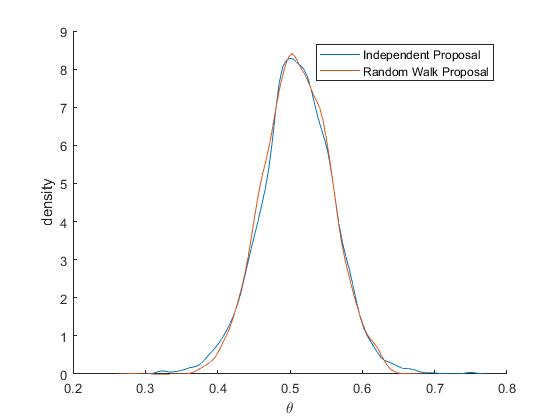
\includegraphics[scale = 0.5]{binomial_comparison.jpg}
%\end{subfigure}
\caption{\textit{Comparison of standard random walk and independent proposals for binomial example}}
\end{figure}

\paragraph{}
Above figure was produced with (N = 15000) particles with a true $\theta$ value of 0.5 and 51 successes for the observed data. Clearly both proposal methods produce reasonable posteriors and they are approximately equivalent.
\par

\begin{table}[H]
\begin{center}
\begin{tabular} { | c | c | c | c | c | }
\hline
 & run no. & no. simulations  & run time & estimated mean \\
\hline
\multirow{3}{7em}{Random Walk Proposals} & 1 & 157278 & 16s  & 0.5053\\
 & 2 & 143529 & 14s & 0.5075\\
 & 3 & 126002 & 12s & 0.5082\\
\hline
\multirow{2}{7em}{Independent Proposals} & 1 & 227500 & 109s & 0.5103\\
 & 2 & 190000 & 92s & 0.5088\\
 & 3 & 226250 & 103s & 0.5069\\
\hline
\end{tabular}
\caption{\textit{Comparison of standard random walk proposals and independent proposals for binomial example}}
\end{center} 
\end{table}

\paragraph{}
The above table was produced with (N = 4000) particles. The estimated $\theta$ are all reasonably close to the true value of 0.5 with 51 successes recorded for the observed dataset. There are three factors that are believed to be the cause for the increased computation time for the independent proposal method. The main cause is having to compute the proposal density for the independent proposal. For the standard random walk the proposal density is not needed as the terms cancel due to the proposal being symmetric while for the independent proposal it is needed twice for every proposed $\boldsymbol{\theta}$. Secondly, as the proposal density needs to be calculated early rejection is no longer possible which results in more simulations needed to be run. Thirdly, there may be some increased computation around saving all proposed thetas and their score and proposal density. 
\par
%
%Transform: 
%A reasonable suggestion for the proposal distribution would be a normal random walk (WORDING CORRECT?). However, if applied to theta (which only has a range between 0 and 1) many proposals will be made outside of this range which would be inefficient. Instead we want to transform $\theta$ to a parameter that covers the range $-\inf < \phi < \inf$. The transformation used was $\phi \sim  ln(\frac{\theta}{1 - \theta})$.


%(Mention MCMC approach briefly)
%SMC approach: Random walk, Independent proposals
%
%
%Random walk: 
%$q(\theta*|\theta)$ is an arbitrary proposal over the $\theta$ space. When the proposal is symmetric such normal random walk terms cancel.
%Independent proposal: 
%Non-parametric, sum of normal distributions around data points.
%
%Transform:




\subsection{G-and-k example}
\subsubsection{Model and Data}
\paragraph{}
Both SMC ABC proposal methods were applied on the g-and-k distribution described in \citeA{drovandi2015} and \citeA{rayner}.
This is a quantile distribution which can be defined in terms of its quantile function. Such functions can be formulated to create more flexible distributions than other standard distributions. This quantile function, which can also be interpreted as a transformation of a standard normal random variate, has the following form:
\par
\begin{equation*}
Q(z(p); \boldsymbol{\theta} ) = a + b \left( 1 + c\frac{1 - exp(-gz(p))}{1 + exp(-gz(p))}	\right) (1 + z(p)^2 )^k z(p)
\end{equation*}
\paragraph{}
Here $p$ denotes the quantile of interest while $z(p)$ represents the quantile function of the standard normal distribution. The model parameter is $\boldsymbol{\theta} = (a, b, c, g, k)$, though common practice is to fix c at 0.8 \cite{rayner}. While the likelihood function can be computed numerically, it is much more expensive than simulating from the model which can be cheaply implemented for quantile distributions via the inversion method.
\par

\paragraph{}
The observed dataset consists of 10000 independent draws from the g-and-k distribution with $a = 3, b = 1, c = 0.8, g = 2 and k = 0.5$. \citeA{drovandi2015} suggests using three component normal mixture model with 8 parameters as an auxiliary model. A mixture model is a suitable choice for an auxiliary distribution as it can be made arbitrarily flexible while maintaining a tractable likelihood function.
\par

\paragraph{}
An efficient discrepancy function is the Mahalanobis distance:
\begin{equation*}
\rho(y, x) = (S(y) - S(x))^T W (S(y) - S(x)),
\end{equation*}
where W is a 'weighting' matrix that takes into account the scale of the summaries and the correlations between summaries. For this example the discrepancy function takes the form:
\begin{equation*}
\rho(y, x) = S_A(x, \phi_y)^T J(\phi_y)^{-1} S_A(x, \phi_{obs})
\end{equation*}
where $J(\phi_y)$ is the weighting matrix based on the estimated covariance matrix of the auxiliary parameter estimates.
\par

\subsubsection{Results}

\begin{table}[H]
\begin{center}
\begin{tabular} { | c | c | c | c | c | c | c | c |}
\hline
 & run no. & no. simulations  & run time & $\hat{a}$ &  $\hat{b}$ &  $\hat{g}$  &  $\hat{k}$\\
\hline
\multirow{6}{7em}{Random Walk Proposals} & 1 &   & 745s & 2.996 & 1.012 & 2.043 & 0.486  \\
& 2 & 2527577 & 714s & 2.998 & 1.023 & 2.073 & 0.485\\
& 3 & 1273216 & 198s & 2.997 & 1.022 & 2.063 & 0.479\\
& 4 & 1290764& 236s & 2.996 & 1.026  & 2.066 & 0.477\\
& 5 & 2529751 & 983s & 3.000 & 1.025 & 2.050 & 0.480\\
& 6 & 2652931 & 575s & 2.998 & 1.026 & 2.061 & 0.481\\
\hline
\multirow{6}{7em}{Independent Proposals} & 1 & 828800  & 1894s & 2.998 & 1.019 & 2.046 & 0.481 \\
& 2 & 1028000 & 4423s & 2.994 & 1.012 & 2.049 & 0.483\\
& 3 & 1228000 & 6286s & 2.997 & 1.025 & 2.075 & 0.479\\
& 4 & 1171200 & 7549s & 3.049 & 1.099  & 2.203 & 0.457\\
& 5 & 760800 & 2658s & 3.003 & 1.028 & 2.050 & 0.478\\
& 6 & 1291600 & 6244s & 2.997 & 1.022 & 2.060 & 0.480\\
\hline 
\end{tabular}
\caption{\textit{Comparison of standard random walk proposals and independent proposals for g-and-k example}}
\end{center} 
\end{table}

\paragraph{}
The above data was produced with (N = 800) particles. Both proposals give reasonable estimates for true parameter values (a = 3, b = 1, g = 2, k = 0.5). The reasons for the increased computation time for the independent proposal method are the same as outlined in the binomial example.
\par

%\paragraph{}
\begin{figure}[H]
\centering
\begin{subfigure}{6cm}
\centering
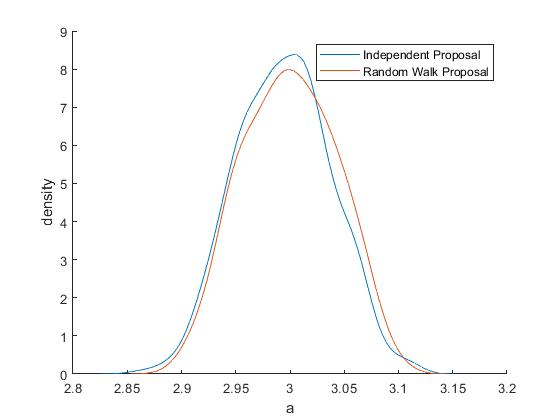
\includegraphics[width=6cm]{gandk_comparison_a.jpg}
\end{subfigure}
\begin{subfigure}{6cm}
\centering
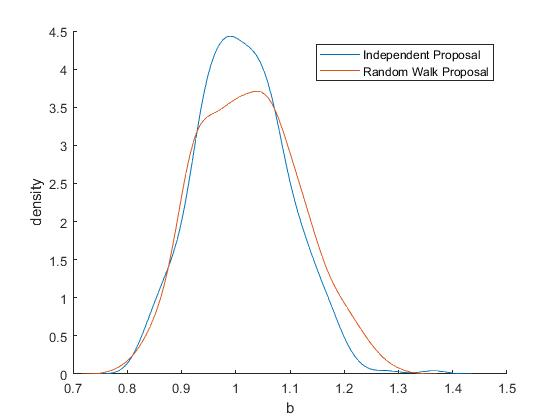
\includegraphics[width=6cm]{gandk_comparison_b.jpg}
\end{subfigure}
\begin{subfigure}{6cm}
\centering
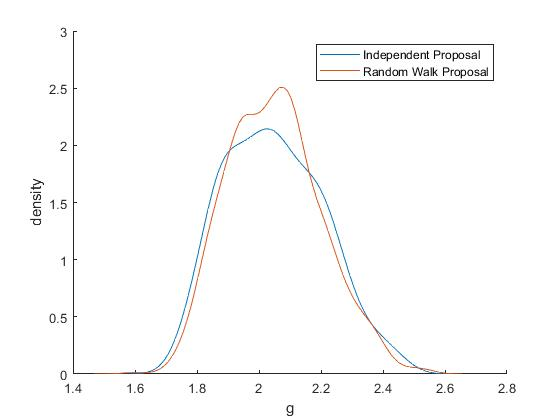
\includegraphics[width=6cm]{gandk_comparison_g.jpg}
\end{subfigure}
\begin{subfigure}{6cm}
\centering
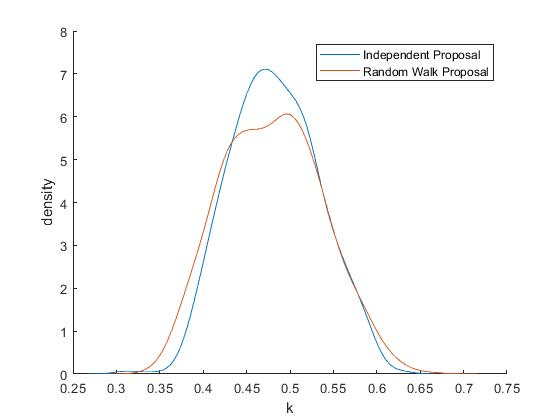
\includegraphics[width=6cm]{gandk_comparison_k.jpg}
\end{subfigure}
\caption{\textit{Comparison of approximate posteriors for proposal methods}}
\end{figure}
%\par

\paragraph{}
Both methods were run with (N = 800) particles and a minimum acceptance rate of 0.5\%. Reasonable to expect both methods to produce the even more similar posteriors as the number of particles increases. 
\par

\begin{figure}[H]
\centering
\begin{subfigure}{6cm}
\centering
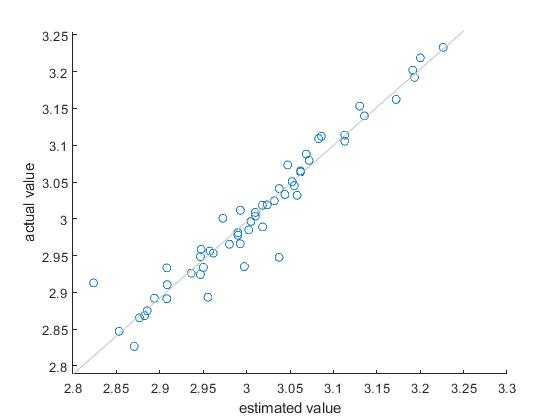
\includegraphics[width=6cm]{gk_est_a.jpg}
\caption{a}
\end{subfigure}
\begin{subfigure}{6cm}
\centering
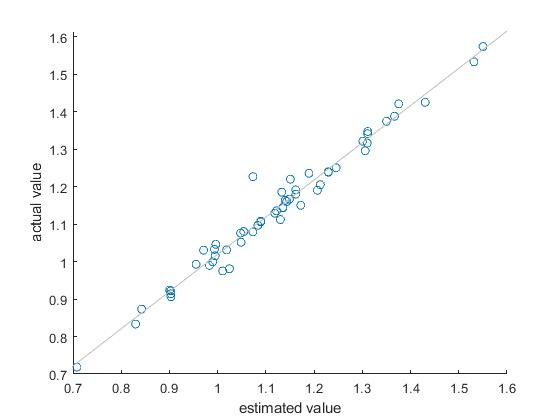
\includegraphics[width=6cm]{gk_est_b.jpg}
\caption{b}
\end{subfigure}
\begin{subfigure}{6cm}
\centering
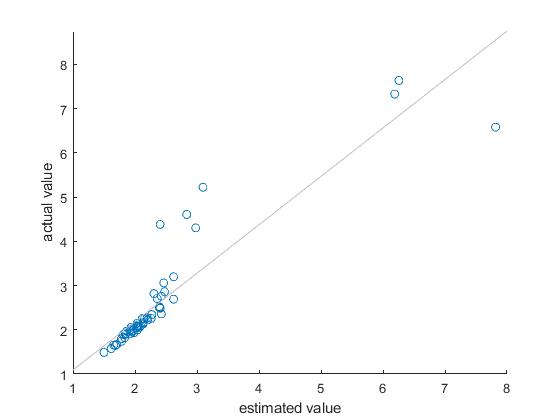
\includegraphics[width=6cm]{gk_est_g.jpg}
\caption{g}
\end{subfigure}
\begin{subfigure}{6cm}
\centering
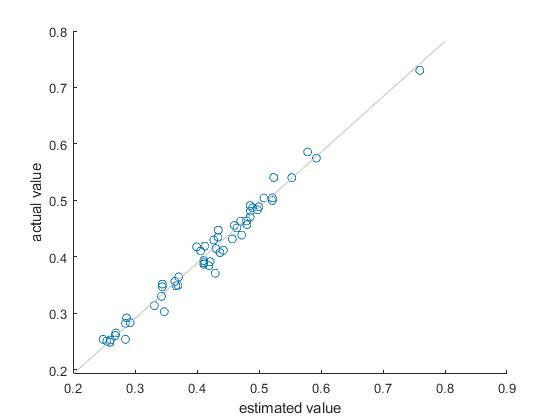
\includegraphics[width=6cm]{gk_est_k.jpg}
\caption{k}
\end{subfigure}
\caption{\textit{estimated parameters against true parameters}}
\end{figure}


\paragraph{}
The final set of parameters were saved after a SMC ABC run on the g-and-k model. A value, $\theta_r$, was randomly selected and a dataset was simulated. The algorithm was then run with (N = 750) particles for 60 times. While the parameters a, b, and k are well estimated there appears to be some problems with the parameter g. This is due to the presence of a small number of particle with a much higher value. A small $\epsilon$ value is needed to stop values clustering around this point. Running with a higher number of particles and a lower acceptance rate threshold will likely resolve the issue.  
\par


%	\paragraph{}
%How recycling was applied:
%Every theta that was proposed and its corresponding proposal density and score was recorded. 
%\par

\section{Discussion}
\paragraph{}
In this report, SMC ABC with independent proposal was implemented and shown to give a good estimate of the true parameters. It was also shown that the approximate posterior was approximately the same as when using SMC ABC with a normal random walk proposal.  The two methods were first applied on a trivial example of a binomial distribution and then on a more computationally intensive g-and-k model. The independent proposal method required more time to run for a single dataset. However, implementing this approach allows for further work to be done by recycling the independent proposals saved which will result in a higher ESS. 
\par

\paragraph{}
Computation was limited by no access to high performance computing with all results run on standard computers. Due to time constraints this limited the number of particles, number of data points simulated, acceptance rate and the number of times the method was run.
 \par

\paragraph{}
More steps needed to fully implement independent proposal recycling for the g-and-k example. By using all proposed particles instead of the final samples $\{ \boldsymbol{\theta}^i_T \}^M_{i=1}$ a higher ESS can be achieved. Additionally, it can then be determined what approach is more efficient, possibly by taking the average effective sample size (ESS, averaged over the four parameters in the G-ank-K example) divided by the computation time. 
\par




\appendix

%\bibliographystyle{plain}
\setlength{\bibleftmargin}{.125in}
\setlength{\bibindent}{-\bibleftmargin}

\bibliography{vres_bibliography}
%\bibliographystyle{plain}



\end{document}










